\section{Nuclear Models}
\begin{itemize}
    \item Two main categories, single particle, and collective. 
    \item Collective models looks at the nucleas as a whole. Single particle models looks at the nucleas as a collection of individual particles.
\end{itemize}

\subsection{Liquid-Drop Model}
\begin{itemize} 
    \item A collective model. 
    \item Assumes the nucleus behaves like molecules in an oscillating drop of liquid.
    \item All molecules attract eachother and are held together by surface tension. 
    \item The droplet is charged which destabilizes the oscillations. 
    \item Heavy droplets are shaped like dumbbells, as they are almost split in two. 
    \item The models explains the binding energy and mass of the nuclei. It also explains the fission of heavy nuclei.
    \item The model does not explain the shell structure or magic numbers  
\end{itemize}

\subsection{Fermi-Gas model \cref{fig: Fermi-Gas_model}}
\begin{itemize}    
    \item A single particle model.
    \item Consider a system of completely non-interacting nucleons in a three dimensional box potential. 
    \item The potential is a well-potential, which treats protons and neutrons differently. The protons has a lower potential than the neutrons. 
    \item The nucleons are arranged in pairs because of the Pauli exclusion principle. 
    \item The Fermi energy $E_{F}$ is the energy of the highest occupied state.
    \item The Fermi momentum $p_{F}$ is the momentum of the highest occupied state.
    \item To calculate $E_{F}$, we must first calculate the number of states in the box of volume $V$. 
    \begin{equation}
      \mathrm{d}A = 4 \frac{V}{Δx^3}
    \end{equation}
    \item The model can not explain the shell structure or magic numbers.
    
    \begin{figure}[h!]
    \centering
    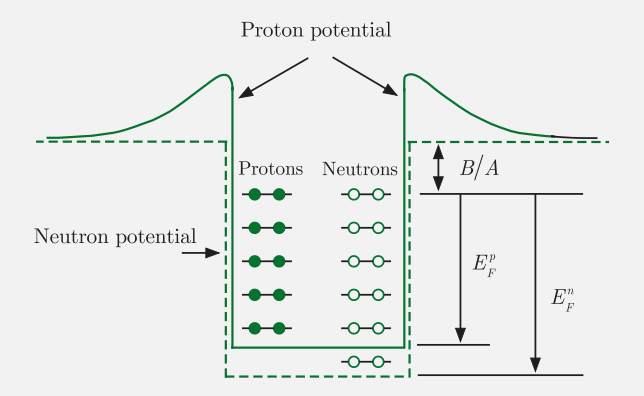
\includegraphics[width = .55\textwidth]{Fermi-Gas_model.png}
    \caption{Visual representation of the Fermi-Gas model}
\end{figure}
    \label{fig: Fermi-Gas_model}
\end{itemize}

\subsection{Shell Model \cref{fig: shell_model_energy_levels}}
\begin{itemize}
    \item A single particle model. Takes inspiration from the shell structure of the atom. 
    \item Explains the shell structure and properties of nuclei. Explains the magic numbers 
    \item The model assumes the particles do not interact. They are affected by a radial central spherical potential created by all the nucleons. It is therefore easier to estimate the movement of any single nucleon. 
    \item Nuclei with magic numbers are more stable. The magic numbers for protons are 2, 8, 20, 28, 50, 82. The magic numbers for neutrons are 2, 8, 20, 28, 50, 82, 126.
    \item Double magic nuclei are nuclei with magic numbers for both protons and neutrons.
    \item Instead of just having the nucleons pair up as in the Fermi-Gas model, the nucleons are arranged in shells.
    \item Each shell has a maximum number of nucleons.
    \item When certain magic number are reached, the separation energy is higher. They are therefore more stable.
    \item The electric quadrupole moment is the lowest for nuclei with magic numbers. This hints at them having a spherical shape, which is the most stable shape.
    \item Odd-Odd (Z-P) nuclei have only 4 stable isotopes. 
    \item Odd-Even nuclei have 50 stable isotopes.
    \item Even-Odd nuclei have 53 stable isotopes.
    \item Even-Even nuclei have 165 stable isotopes.
    
    \begin{figure}[h!]
    \centering
    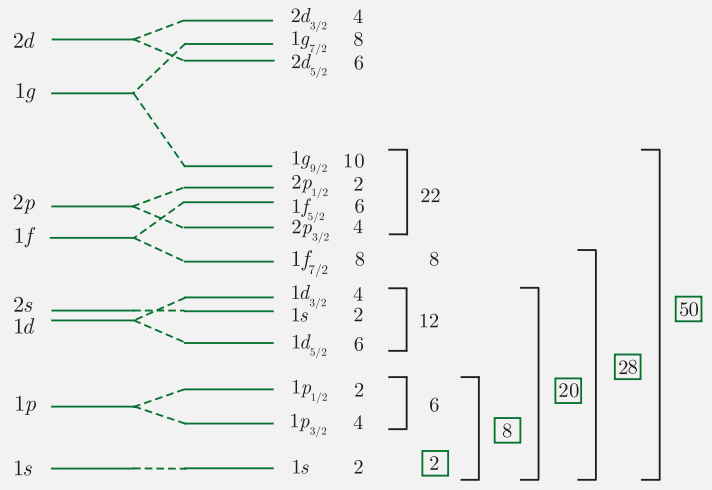
\includegraphics[width = .75\textwidth]{shell_model_energy_levels.png}
    \caption{Lowest energy levels for nucleons with their spin-orbit term.}
    \label{fig: shell_model_energy_levels}
    \end{figure}
    
\end{itemize}

\subsubsection{Simplifying the Complex System to a Simple Model \cref{fig: central_pot_simplification}}
\begin{figure}[h!]
\centering
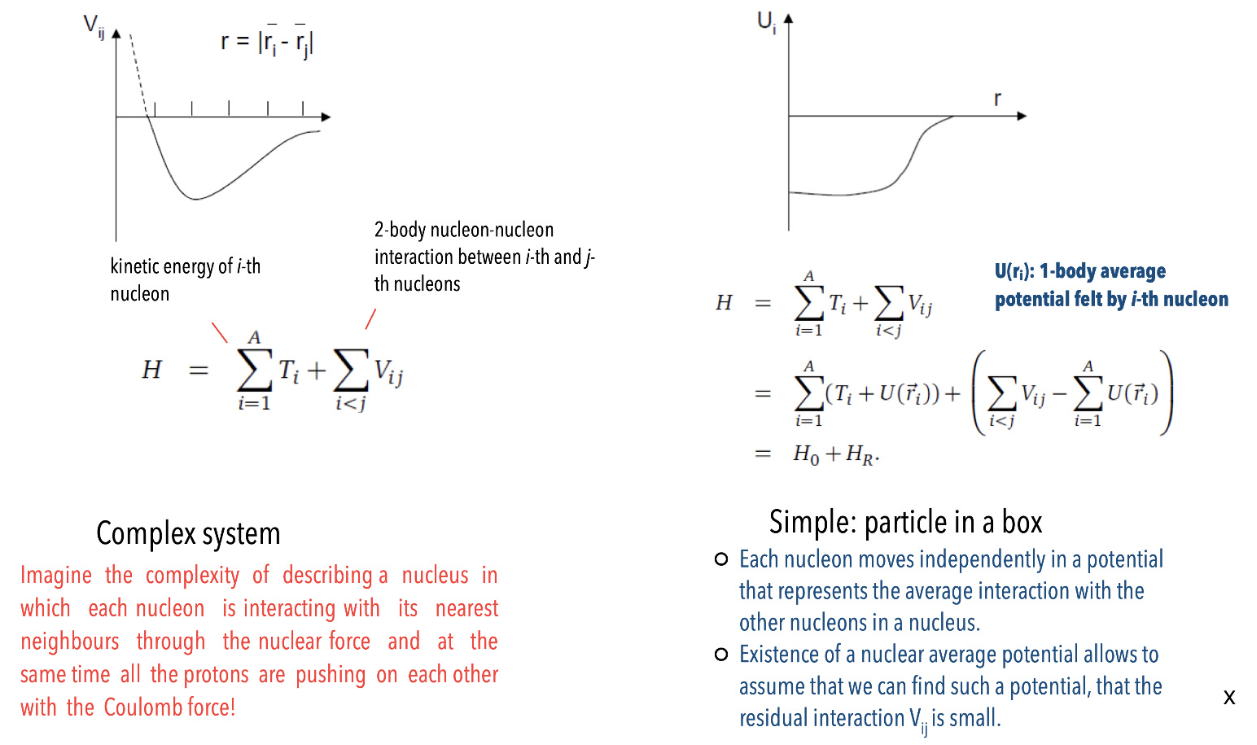
\includegraphics[width = .75\textwidth]{central_pot_simplification.png}
\caption{The transition from a complex system where all the particles interact, to a simple model where the nucleons are affected by a radial central spherical potential.}
\label{fig: central_pot_simplification}
\end{figure}


\subsubsection{Finding the Hamiltonian}
\begin{itemize}
    \item The system gets complex fast, when we have multiple unpaired nucleons. The Hamiltonian is then given by:
    \begin{equation}
      H = H_0 + H_{\text{res}}
    \end{equation}
    where $H_0$ is the Hamiltonian for the system with paired nucleons, and $H_{\text{res}}$ is the residual Hamiltonian for the unpaired nucleons. 
    \item To find the Hamiltonian we need the potential $U(r)$ and finally reproduce the magic numbers. 
\end{itemize}